%============================================================
%  Iterated Symmetric Centipede: Five-Strategy Extension
%  Beamer presentation synopsis
%  Compile with: pdflatex ISC_presentation.tex
%============================================================
\documentclass[aspectratio=169]{beamer}

\usetheme{Madrid}
\usecolortheme{default}

\usepackage[utf8]{inputenc}
\usepackage[T1]{fontenc}
\usepackage{amsmath,amssymb}
\usepackage{graphicx}
\usepackage{booktabs}
\usepackage{array}

% Put your figures folder here
\graphicspath{{figures/}}

\title[Iterated Symmetric Centipede]{Iterated Symmetric Centipede:\\A Five-Strategy Evolutionary Analysis}
\subtitle{All-$M$, All-$1$, Grim, Grim-Patient, Grim-Forgiver}
\date{2026}

%============================================================
\begin{document}
%============================================================

\begin{frame}
  \titlepage
\end{frame}

%------------------------------------------------------------
\begin{frame}{Outline}
  \tableofcontents
\end{frame}

%============================================================
\section{The Centipede Game}
%============================================================

\begin{frame}{The One-Shot Centipede Game}
  \begin{columns}
    \column{0.55\textwidth}
      \textbf{Setup}
      \begin{itemize}
        \item Two players alternate along a path of $M$ nodes.
        \item At each node the moving player can \textbf{Pass} or \textbf{Take}.
        \item Taking ends the game; total payoff at node $t$ is $t$.
        \item The taker receives share $p \in (\tfrac{1}{2},1]$; the other gets $1-p$.
      \end{itemize}
      \vspace{6pt}
      \textbf{The paradox}\\
      Backward induction $\Rightarrow$ take at node 1 (SPE).\\
      Yet $(\rho_1,\rho_1)$ is Pareto-dominated by $(\rho_M,\rho_M)$.
    \column{0.42\textwidth}
      \textbf{Symmetric version (OSC)}\\[4pt]
      Randomise who moves first $\Rightarrow$ symmetric expected payoffs.
      Strategy $\rho_m$: \emph{``take at the first opportunity at or after node $m$''}.\\[6pt]
      \textbf{OSC payoff matrix} ($M{=}4$, $p{=}3/4$):
      \[
      A =
      \begin{pmatrix}
        1    & 9/4  & 9/4  & 9/4 \\
        3/4  & 2    & 15/4 & 15/4\\
        3/4  & 5/4  & 3    & 21/4\\
        3/4  & 5/4  & 7/4  & 4
      \end{pmatrix}
      \]
  \end{columns}
\end{frame}

%============================================================
\section{Five Strategies}
%============================================================

\begin{frame}{Five Strategies in the Iterated Game (ISC)}
  The ISC repeats the OSC for $T$ rounds; players observe full history.
  \vspace{6pt}
  \begin{description}
    \item[\textbf{All-$M$}] Always play $\rho_M$. Full cooperator; never punishes.
    \item[\textbf{All-$1$}] Always play $\rho_1$. Full defector; never cooperates.
    \item[\textbf{Grim}] Start with $\rho_M$. At the \emph{first} defection by the opponent, switch to $\rho_1$ \emph{permanently}.
    \item[\textbf{Grim-Patient}] Like Grim, but requires \emph{two consecutive} defections before triggering.
    \item[\textbf{Grim-Forgiver}] Punishes with $\rho_1$ for exactly \emph{two rounds} after each defection, then unconditionally returns to $\rho_M$ --- repeating the loop indefinitely.
  \end{description}
  \vspace{6pt}
  \textbf{Key observation:} All-$M$, Grim, GrimP, GrimF never trigger each other --- they all play $\rho_M$ throughout whenever paired together.
\end{frame}

%============================================================
\section{The Payoff Matrix}
%============================================================

\begin{frame}{The ISC Payoff Matrix ($M{=}4$, $T{=}10$, $p{=}3/4$)}
  \begin{columns}
    \column{0.52\textwidth}
      \[
      C =
      \begin{pmatrix}
        40   & 7.5  & 40    & 40   & 40 \\
        22.5 & 10   & 11.25 & 12.5 & 15 \\
        40   & 9.75 & 40    & 40   & 40 \\
        40   & 9.5  & 40    & 40   & 40 \\
        40   & 9.0  & 40    & 40   & 40
      \end{pmatrix}
      \]
      Rows/columns: All-$M$, All-$1$, Grim, GrimP, GrimF.
    \column{0.45\textwidth}
      \textbf{Three structural facts:}
      \begin{enumerate}
        \item All cooperating strategies earn $TM = 40$ against \emph{each other}. They are \textbf{payoff-equivalent} when All-$1$ is absent.
        \item All-$1$'s payoff against a cooperator depends on how long that cooperator holds out before switching.
        \item GrimF is \textbf{most exploitable}: it cycles back to $\rho_M$ every 3 rounds, so All-$1$ earns $C(2,5)=15 > C(2,4)=12.5 > C(2,3)=11.25$.
      \end{enumerate}
  \end{columns}
\end{frame}

%============================================================
\section{Nash Equilibria \& ESS}
%============================================================

\begin{frame}{Nash Equilibria}
  \begin{block}{Cooperative equilibrium set}
    Any mixture over $\{\text{All-}M, \text{Grim}, \text{GrimP}, \text{GrimF}\}$ is a Nash equilibrium.\\
    This is a \emph{continuum} of NE --- a direct consequence of the payoff degeneracy $C(i,j)=TM$ for all cooperating pairs.
  \end{block}

  \begin{block}{All-$1$ equilibrium}
    $(\sigma_2, \sigma_2)$ is a NE \textbf{if and only if} $p \geq 2/3$.
  \end{block}

  \begin{alertblock}{The critical threshold $p^* = 2/3$}
    \begin{itemize}
      \item $p < 2/3$: defecting is not profitable; cooperation dominates.
      \item $p > 2/3$: the first-mover advantage is large enough for All-$1$ to thrive.
    \end{itemize}
  \end{alertblock}
\end{frame}

\begin{frame}{Evolutionarily Stable Strategies (ESS)}
  \begin{itemize}
    \item \textbf{No pure cooperator is an ESS.}\\
      Because all cooperators earn identical payoffs against each other, none can resist a neutral mutation into another cooperating strategy.
    \item \textbf{No mixed strategy on the cooperative face is an ESS.}\\
      Same reason: the cooperative face $\mathcal{F} = \{x_2 = 0\}$ is neutrally stable, not strictly stable.
    \item \textbf{All-$1$ is an ESS if and only if $p > 2/3$.}\\
      Below the threshold, any cooperating strategy can invade an all-defector population and grow.
  \end{itemize}
  \vspace{6pt}
  \textbf{Implication:} below $p^*$, the system converges to cooperation but the final mix among cooperators is determined by initial conditions and drift --- not by selection.
\end{frame}

%============================================================
\section{Replicator Dynamics}
%============================================================

\begin{frame}{Replicator Dynamics --- Model}
  Large-population, continuous-time model.
  Strategy $m$ grows if its payoff exceeds the population average:
  \[
    \dot{x}_m = x_m \bigl[(C\mathbf{x})_m - \mathbf{x}^\top C \mathbf{x}\bigr]
  \]
  \textbf{Key results:}
  \begin{itemize}
    \item The entire cooperative face $\mathcal{F} = \{x_2 = 0\}$ is a \emph{rest-point set} --- no drift among cooperators.
    \item The only interesting dynamics are in the $x_2$ (All-$1$) direction.
    \item $\mathcal{F}$ is asymptotically stable (w.r.t.\ All-$1$ invasion) iff $p < 2/3$.
  \end{itemize}
\end{frame}

\begin{frame}{Replicator Dynamics --- Time Series}
  \begin{columns}
    \column{0.48\textwidth}
      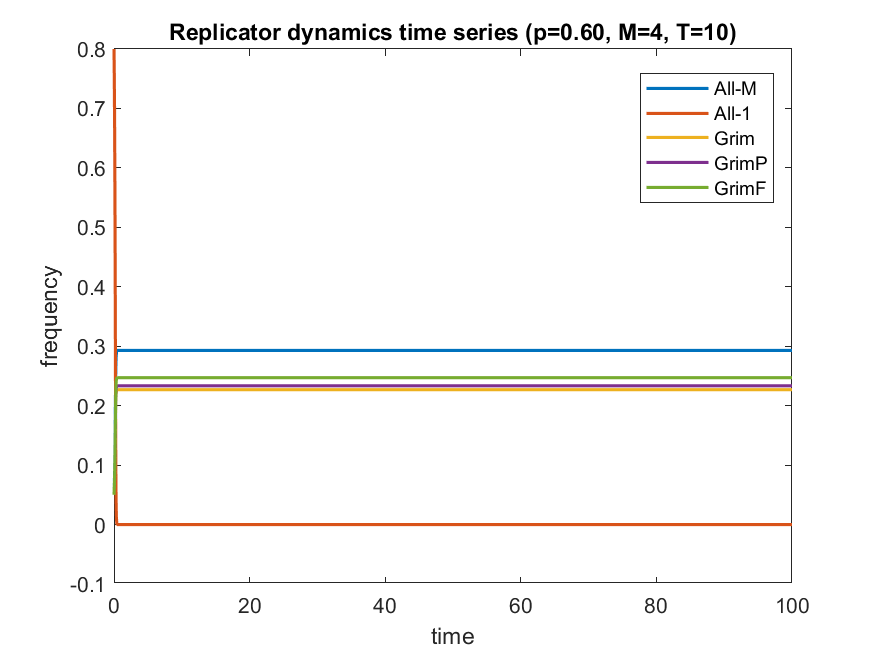
\includegraphics[width=\textwidth]{rep_timeseries_p060}\\
      \centering\small $p = 0.60 < p^*$: All-$1$ driven to zero.
    \column{0.48\textwidth}
      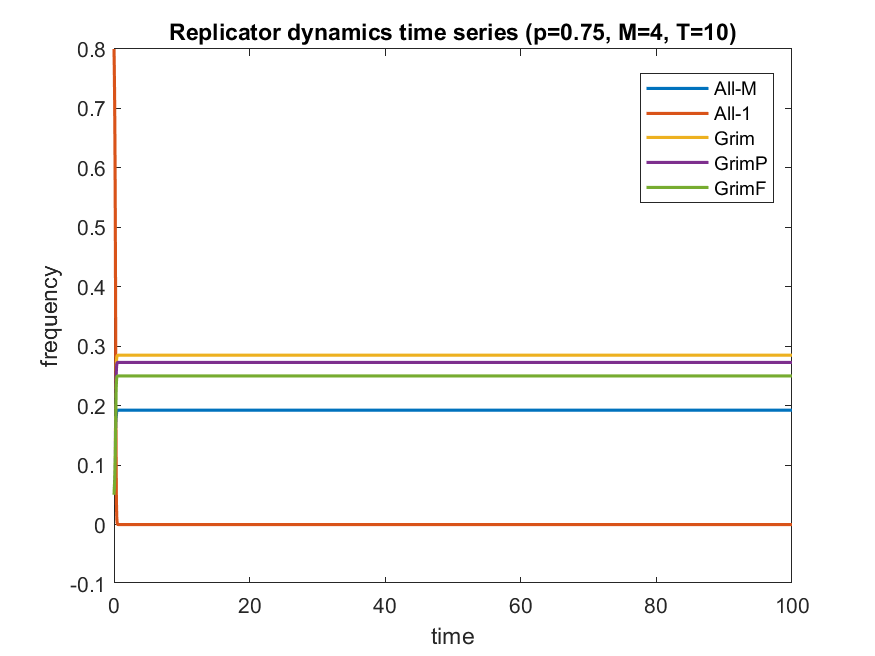
\includegraphics[width=\textwidth]{rep_timeseries_p075}\\
      \centering\small $p = 0.75 > p^*$: All-$1$ remains; cooperators squeezed.
  \end{columns}
  \vspace{6pt}
  \textbf{Note:} equilibrium frequencies are essentially flat --- the dynamics settle very quickly.
\end{frame}

\begin{frame}{Replicator Dynamics --- Phase Portraits}
  Pentagon projection: each vertex = one pure strategy; interior = mixed population.
  \begin{columns}
    \column{0.48\textwidth}
      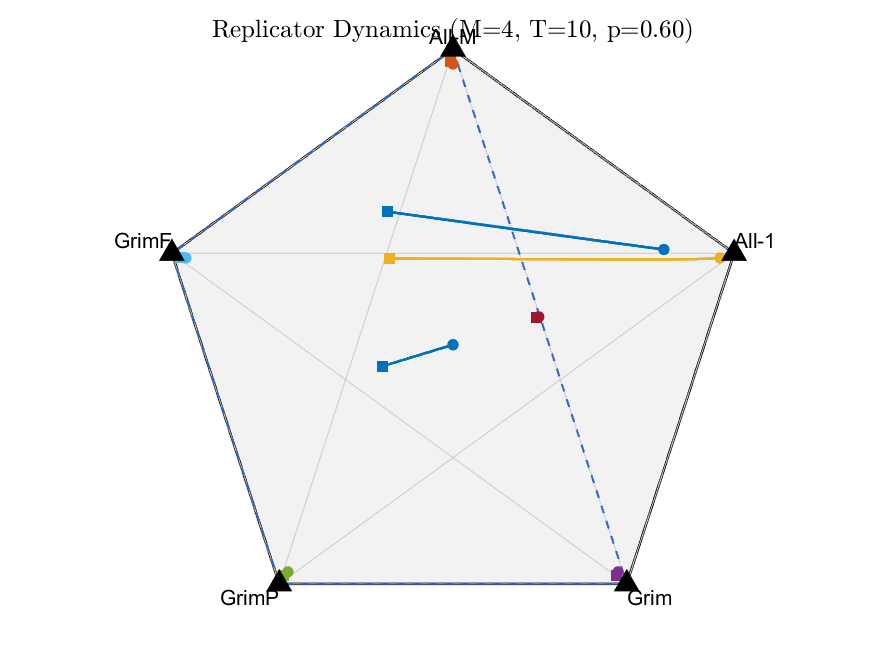
\includegraphics[width=\textwidth]{rep_phase_p060}\\
      \centering\small $p = 0.60$: orbits converge to the cooperative face (away from All-$1$ vertex).
    \column{0.48\textwidth}
      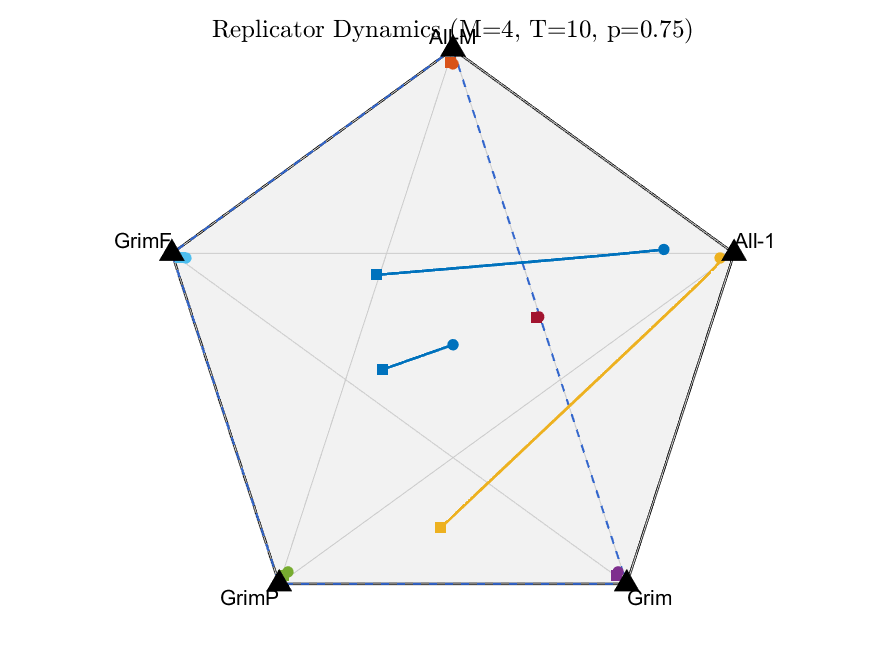
\includegraphics[width=\textwidth]{rep_phase_p075}\\
      \centering\small $p = 0.75$: orbits converge toward the All-$1$ vertex.
  \end{columns}
\end{frame}

\begin{frame}{Replicator Dynamics --- Varying Parameters}
  \begin{columns}
    \column{0.48\textwidth}
      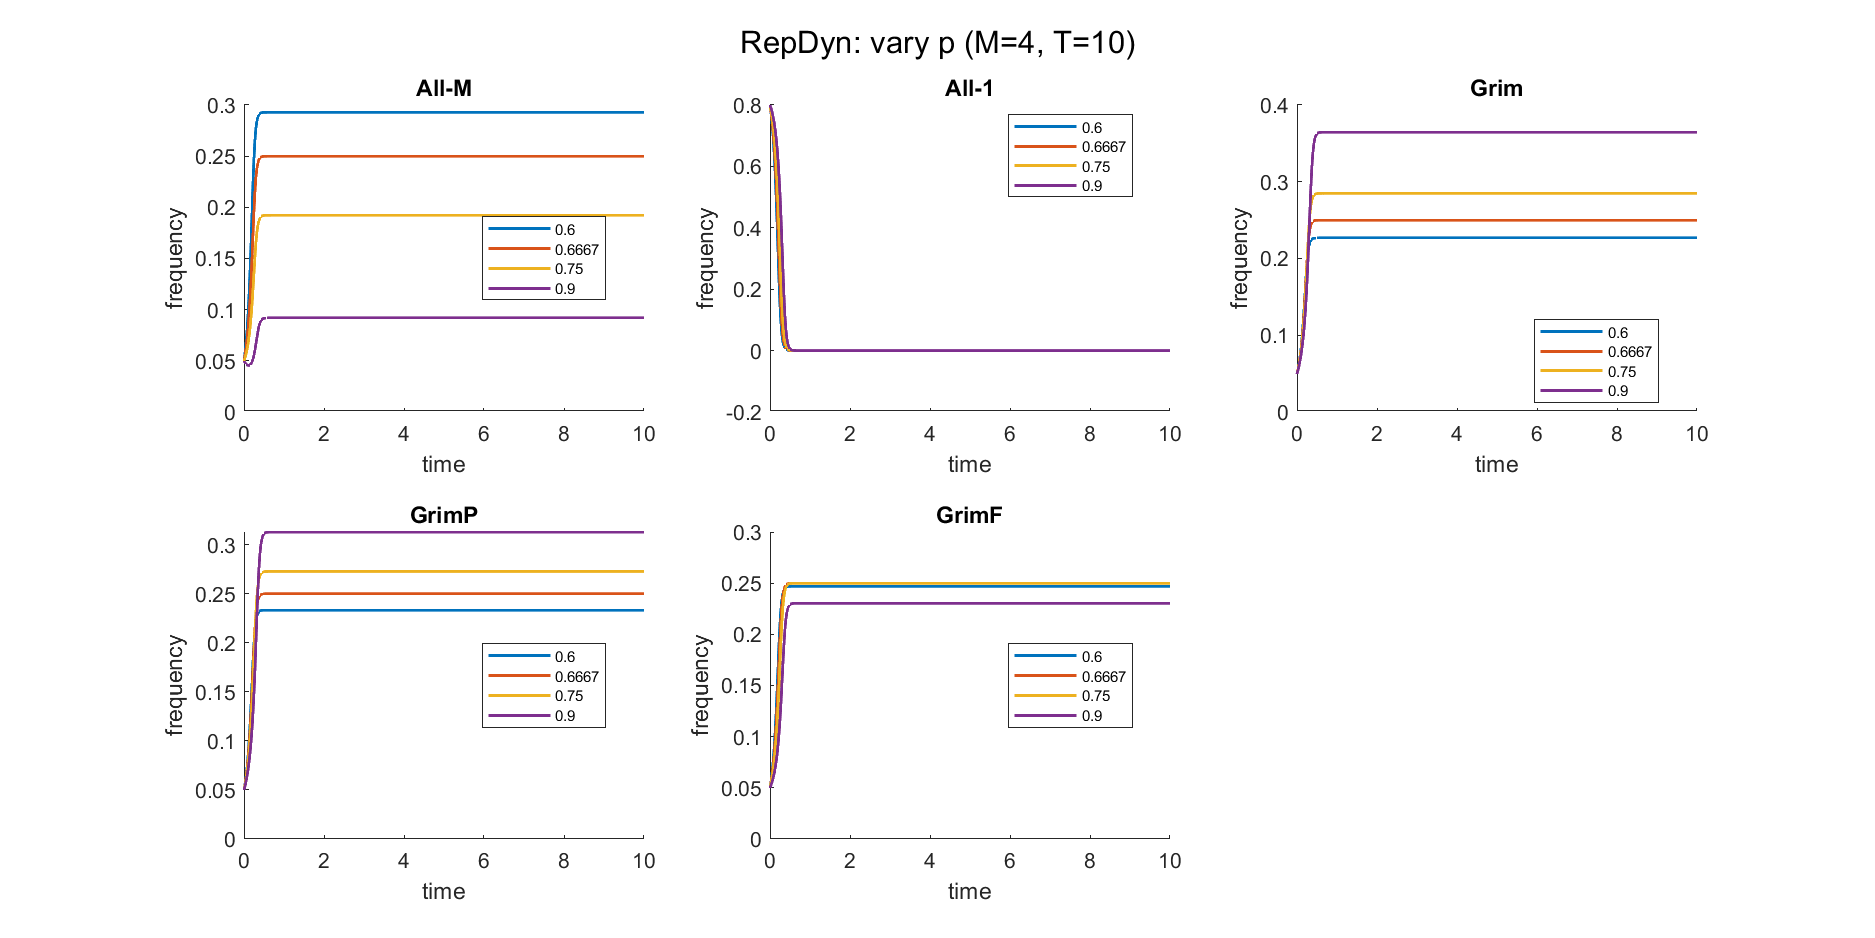
\includegraphics[width=\textwidth]{rep_overlay_vary_p}\\
      \centering\small Vary $p$: threshold at $p^* = 2/3$ clearly visible.
    \column{0.48\textwidth}
      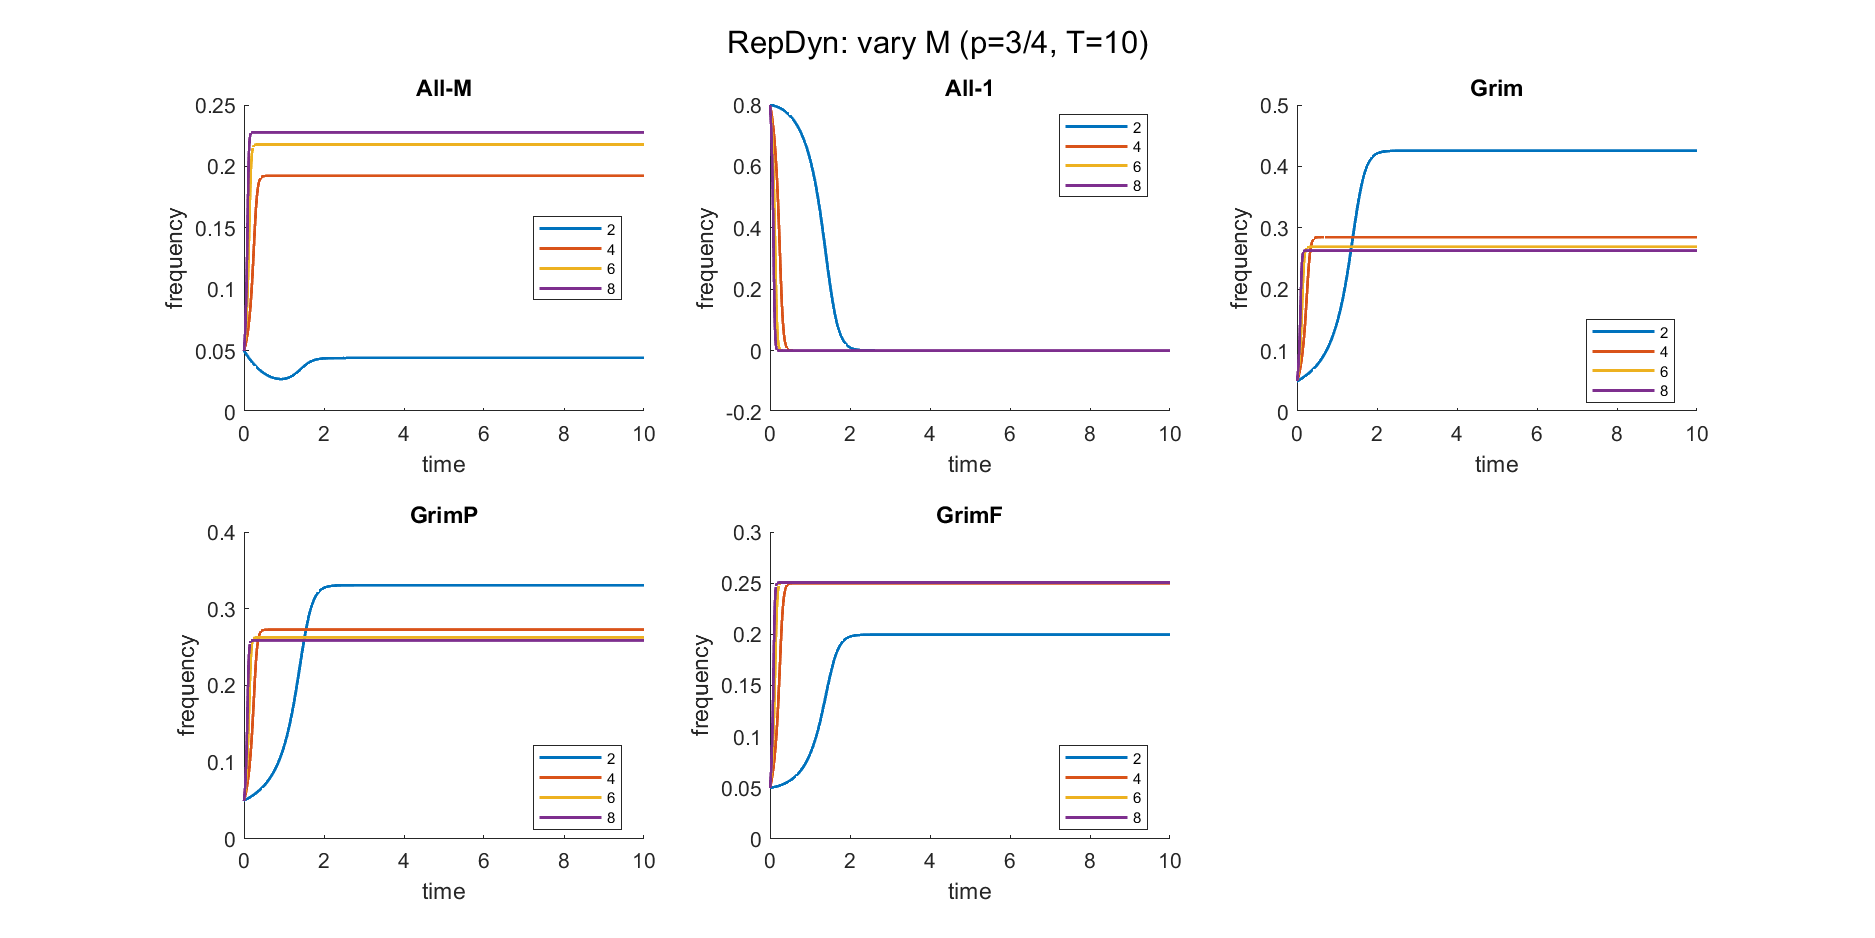
\includegraphics[width=\textwidth]{rep_overlay_vary_M}\\
      \centering\small Vary $M$: larger centipede amplifies cooperation incentives.
    \end{columns}
\end{frame}

\begin{frame}{Replicator Dynamics --- Effect of $T$}
  \begin{center}
    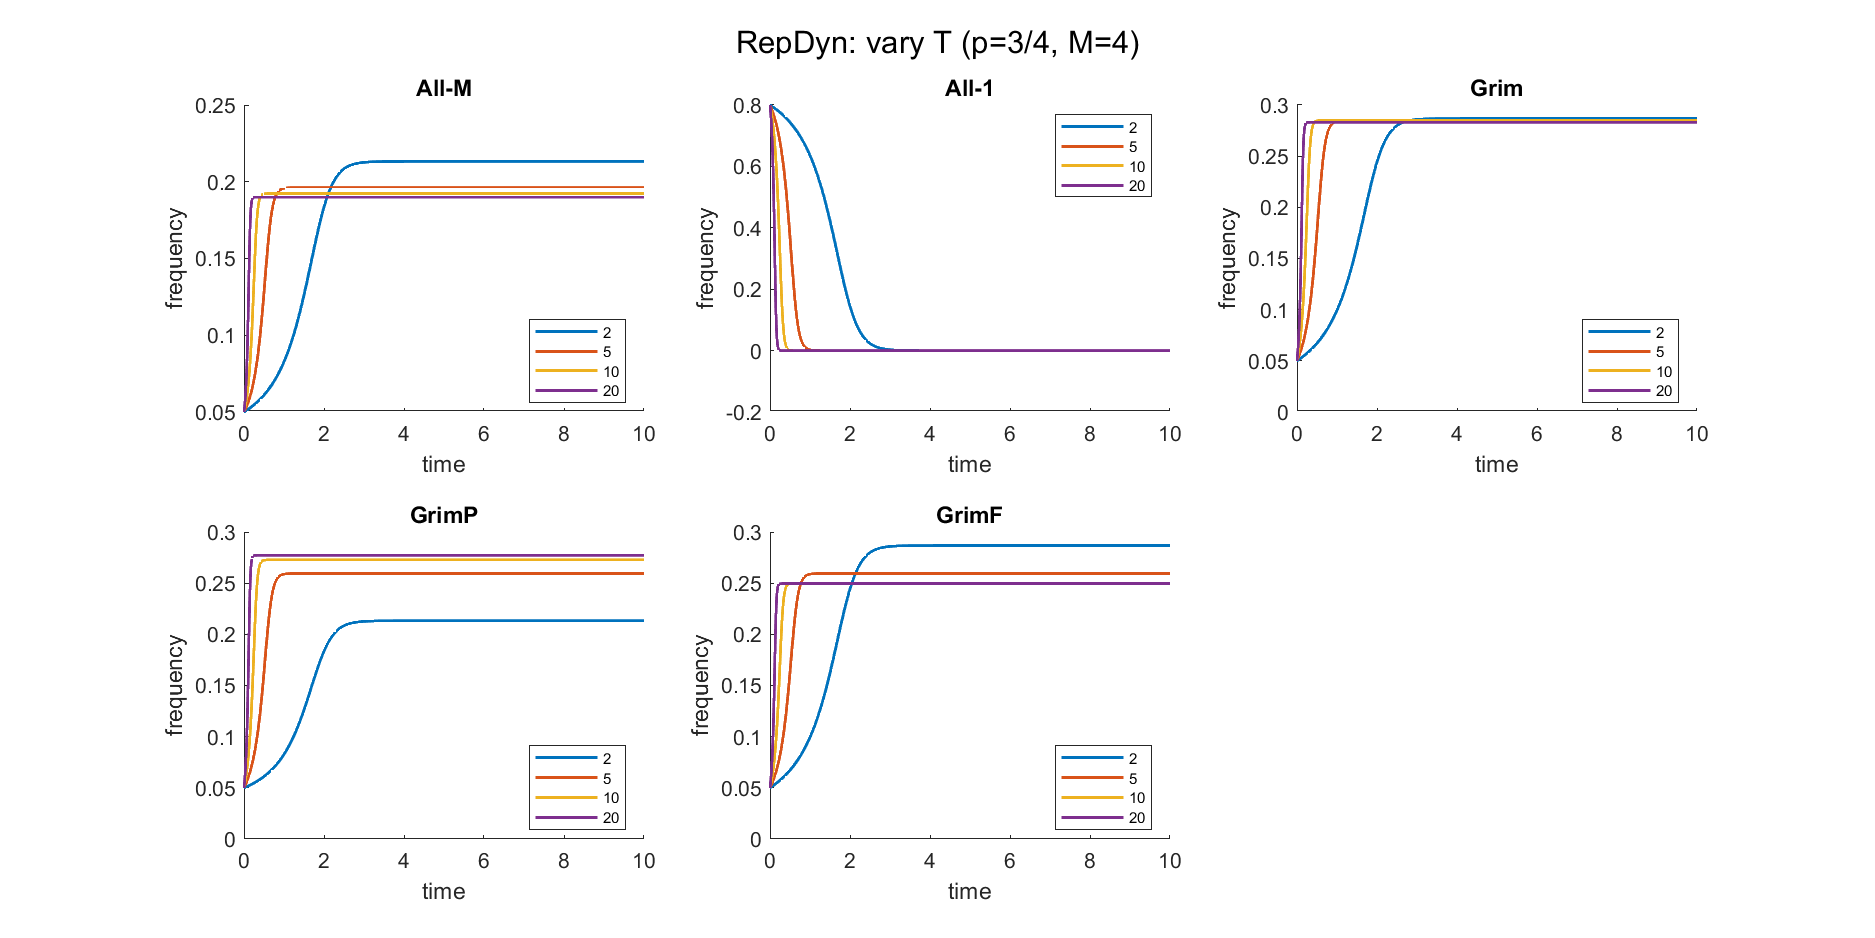
\includegraphics[width=0.65\textwidth]{rep_overlay_vary_T}
  \end{center}
  More repetitions ($T$) mainly affects \textbf{convergence speed}, not the equilibrium frequencies. The long-run outcome is determined by $p$ alone.
\end{frame}

%============================================================
\section{Markov Chain Dynamics}
%============================================================

\begin{frame}{Markov Chain --- Finite Population Model}
  \textbf{Setup:} $N$ agents, each carrying one pure strategy.\\
  At each step: one agent compares payoff with a random opponent and imitates with probability proportional to the payoff difference (\emph{Pairwise Proportional Imitation}).

  \vspace{8pt}
  \textbf{State space:} $(s_1, s_2, s_3, s_4, s_5)$ with $\sum s_i = N$.\\
  Reduced to 2D: $s_M = s_1 + s_3 + s_4 + s_5$ (cooperator count) vs.\ $s_2$ (All-$1$ count).

  \vspace{8pt}
  \begin{block}{Absorbing states}
    \begin{itemize}
      \item The entire \textbf{cooperative face} $\mathcal{A} = \{s_2 = 0\}$: any combination of cooperators with no All-$1$ agents is absorbing.
      \item The \textbf{pure All-$1$} state $(0, N, 0, 0, 0)$.
    \end{itemize}
    All other states are transient.
  \end{block}
\end{frame}

\begin{frame}{Markov Chain --- State Graphs}
  \begin{columns}
    \column{0.48\textwidth}
      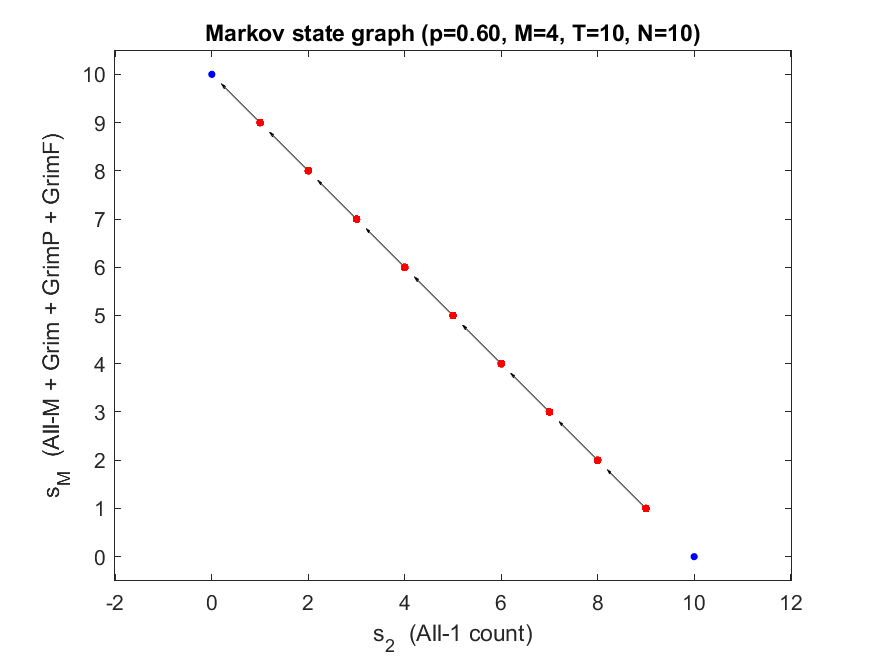
\includegraphics[width=\textwidth]{mark_stategraph_p060}\\
      \centering\small $p=0.60$: drift pushes system toward cooperative face (blue dots = absorbing, red = transient).
    \column{0.48\textwidth}
      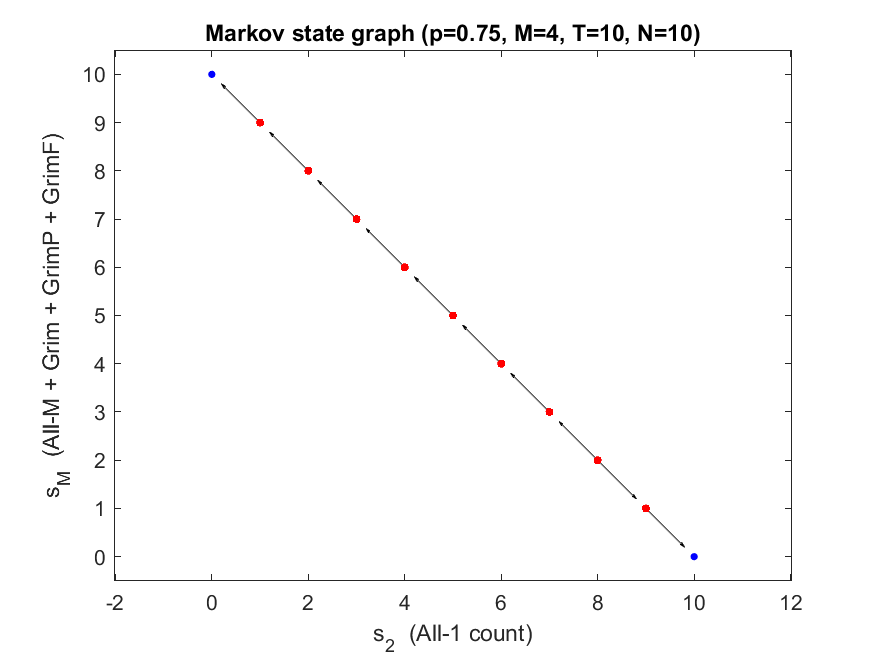
\includegraphics[width=\textwidth]{mark_stategraph_p075}\\
      \centering\small $p=0.75$: both cooperative face and All-$1$ vertex are attractors.
  \end{columns}
\end{frame}

\begin{frame}{Markov Chain --- Time Series}
  \begin{columns}
    \column{0.48\textwidth}
      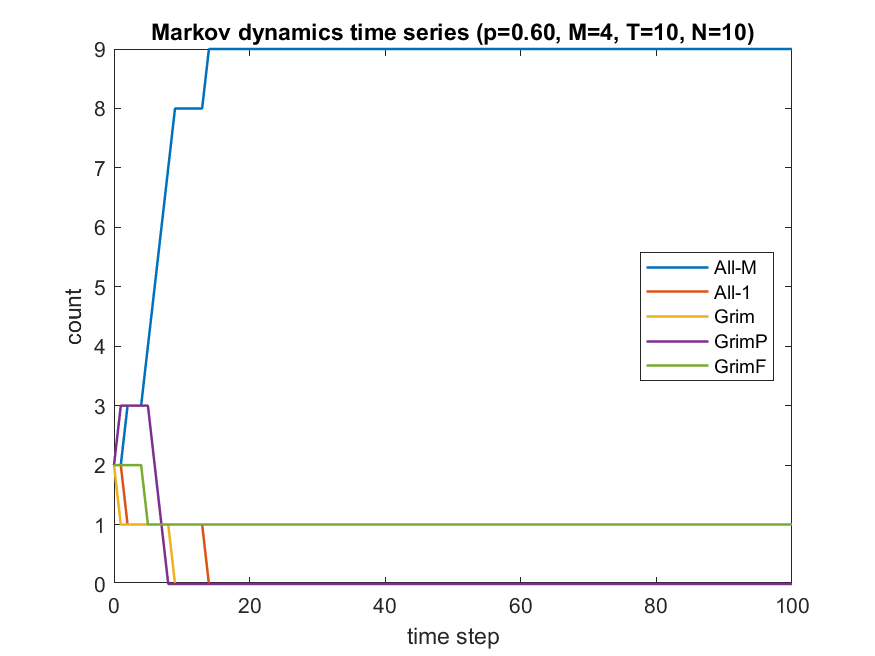
\includegraphics[width=\textwidth]{mark_timeseries_p060}\\
      \centering\small $p=0.60$: All-$M$ dominates; others eliminated.
    \column{0.48\textwidth}
      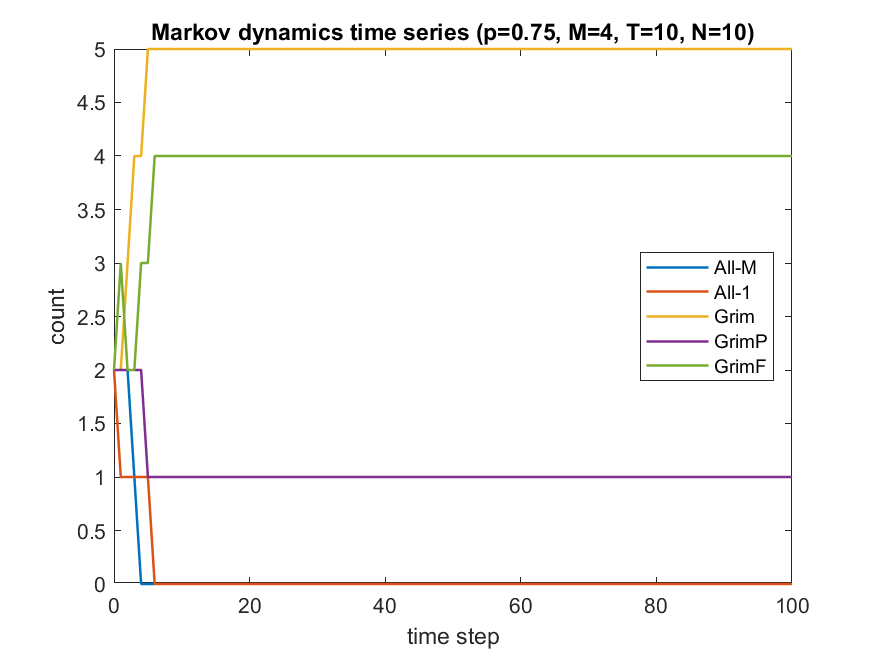
\includegraphics[width=\textwidth]{mark_timeseries_p075}\\
      \centering\small $p=0.75$: GrimF and Grim persist; All-$M$ and All-$1$ collapse.
  \end{columns}
\end{frame}

\begin{frame}{Markov Chain --- Varying Parameters}
  \begin{columns}
    \column{0.48\textwidth}
      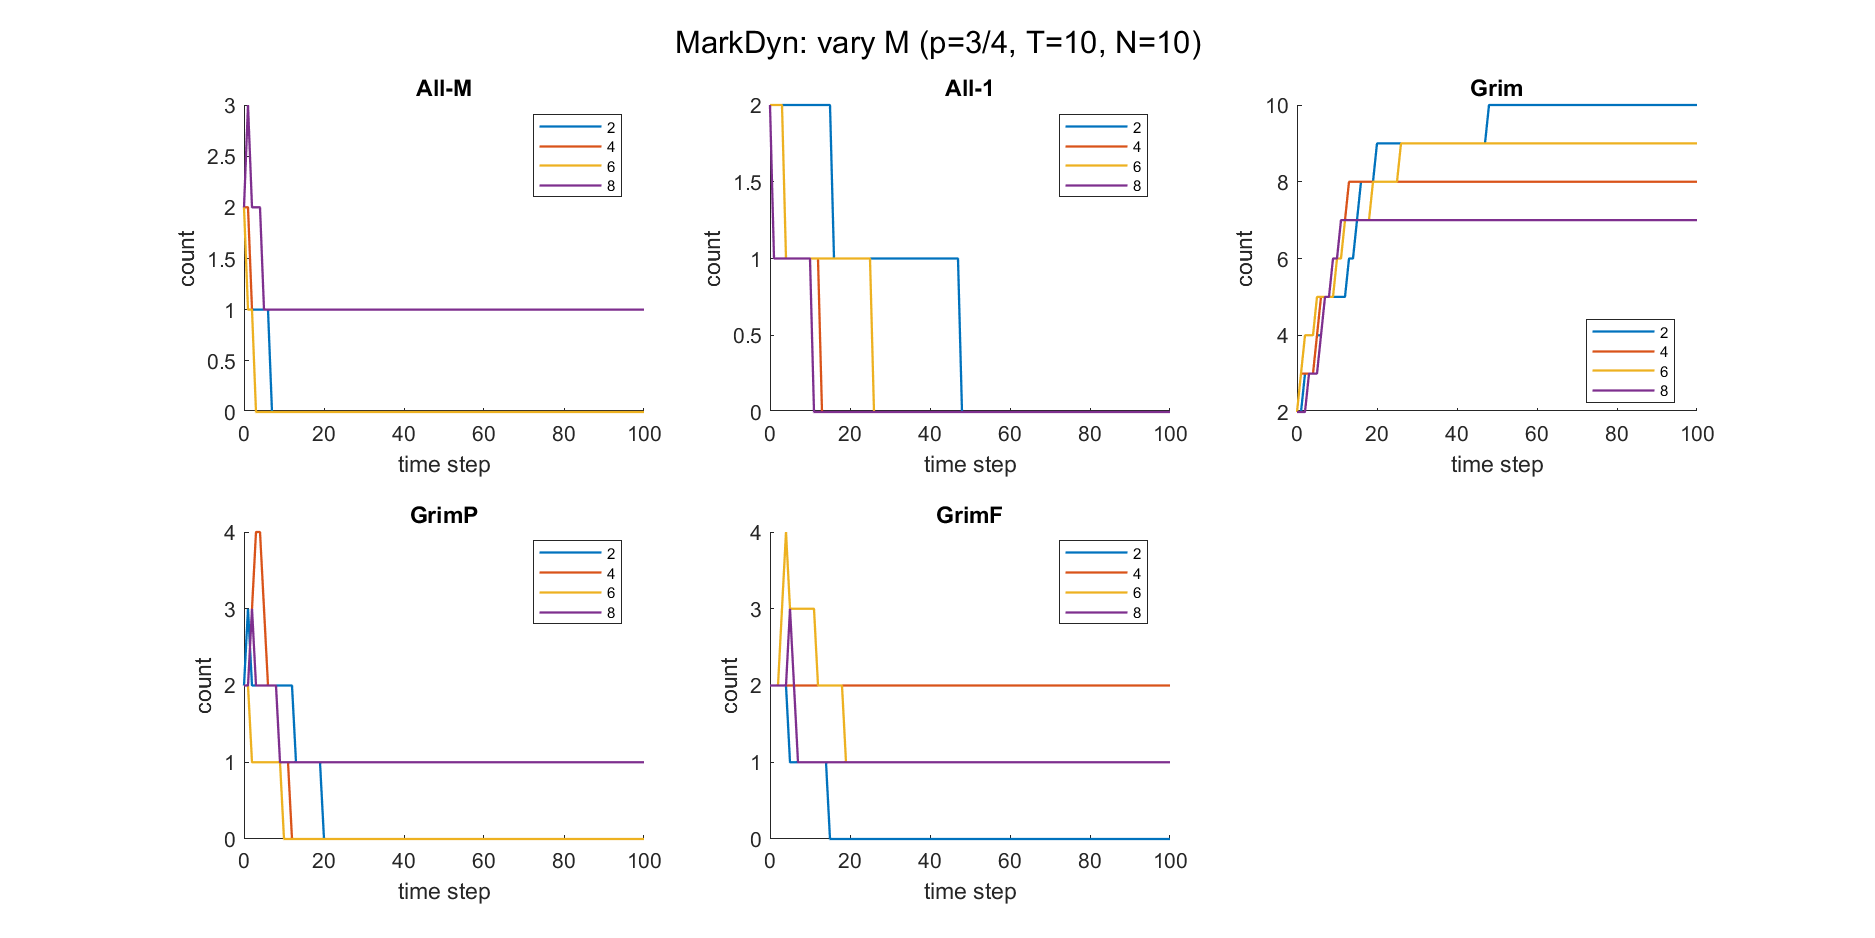
\includegraphics[width=\textwidth]{mark_overlay_vary_M}\\
      \centering\small Vary $M$
    \column{0.48\textwidth}
      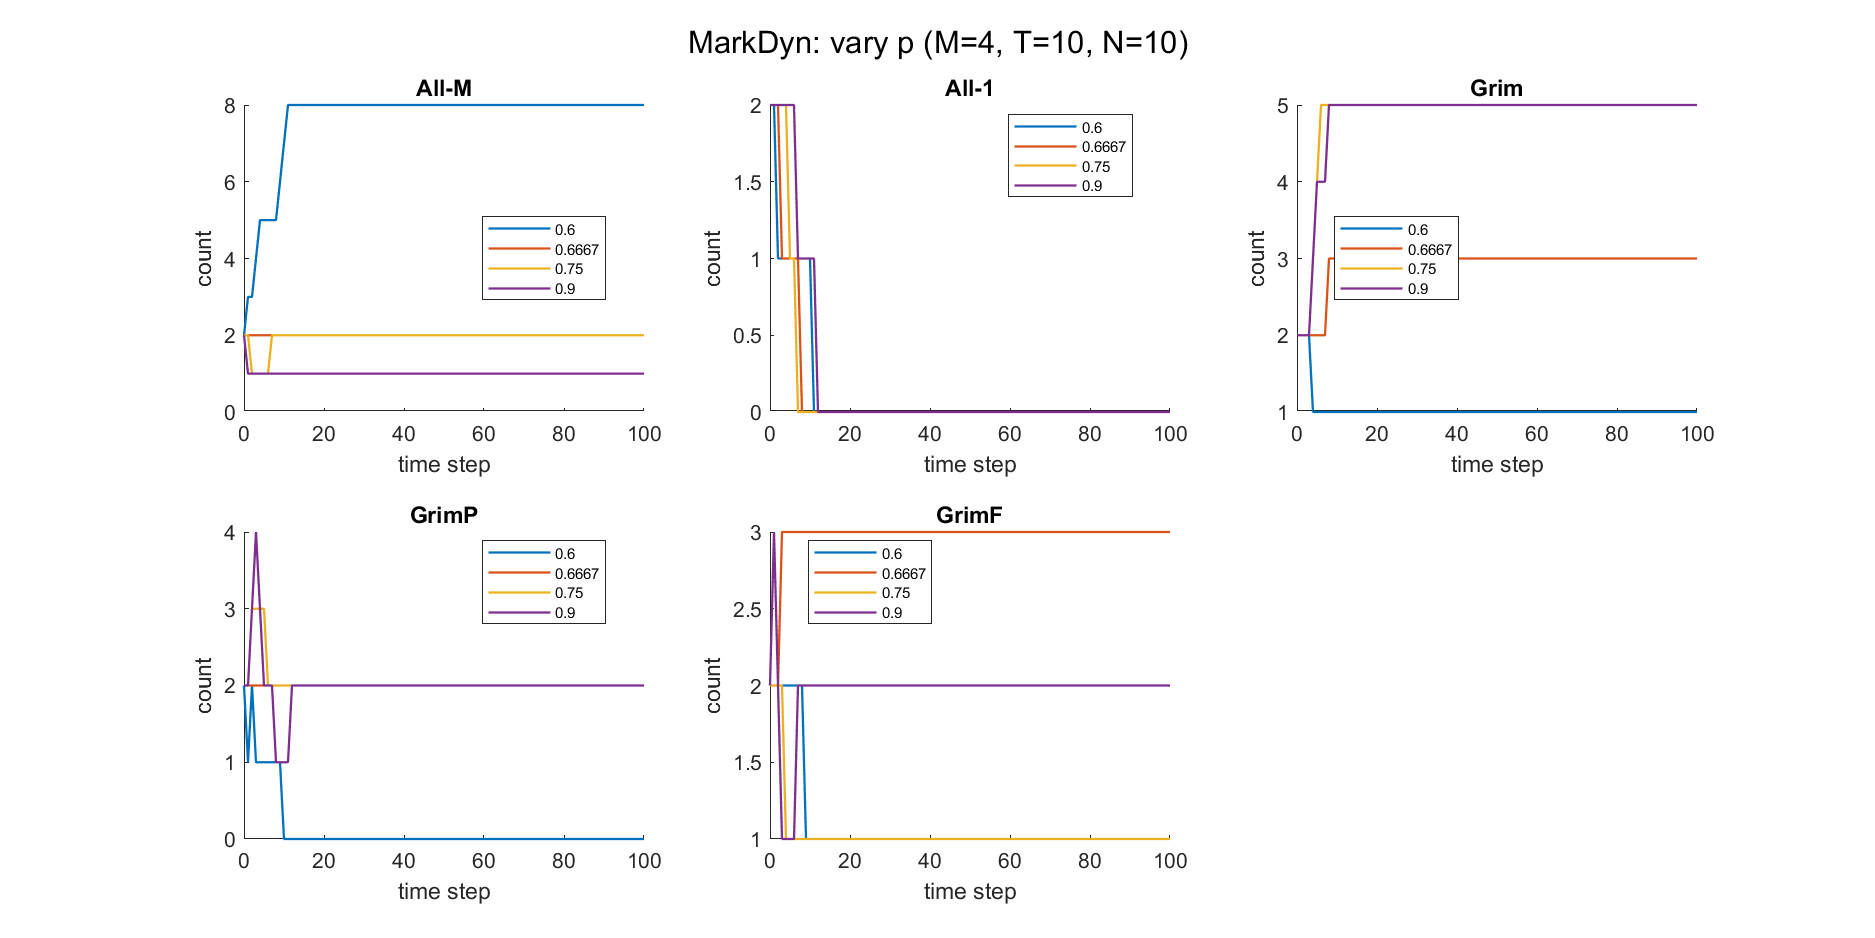
\includegraphics[width=\textwidth]{mark_overlay_vary_p}\\
      \centering\small Vary $p$
  \end{columns}
  \vspace{4pt}
  Larger $M$ strengthens cooperation. Threshold $p^* = 2/3$ again separates the two regimes.
\end{frame}

\begin{frame}{Markov Chain --- Varying $T$ and $N$}
  \begin{columns}
    \column{0.48\textwidth}
      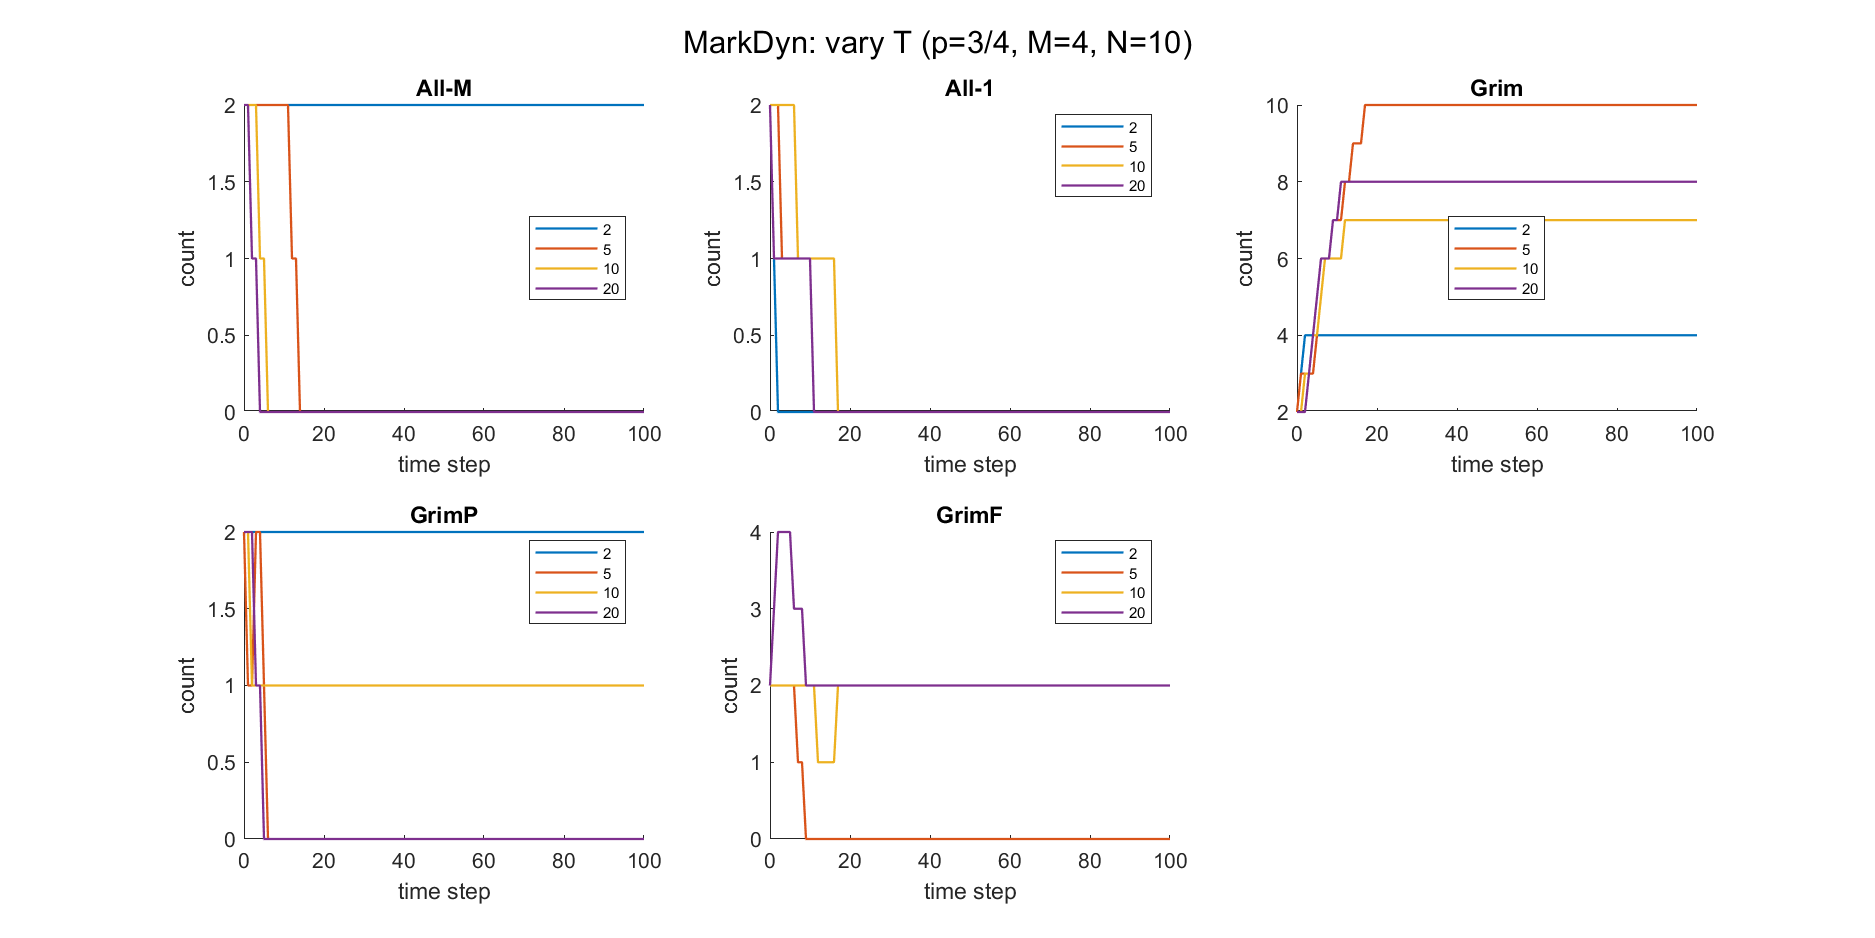
\includegraphics[width=\textwidth]{mark_overlay_vary_T}\\
      \centering\small Vary $T$: more rounds stabilise cooperation.
    \column{0.48\textwidth}
      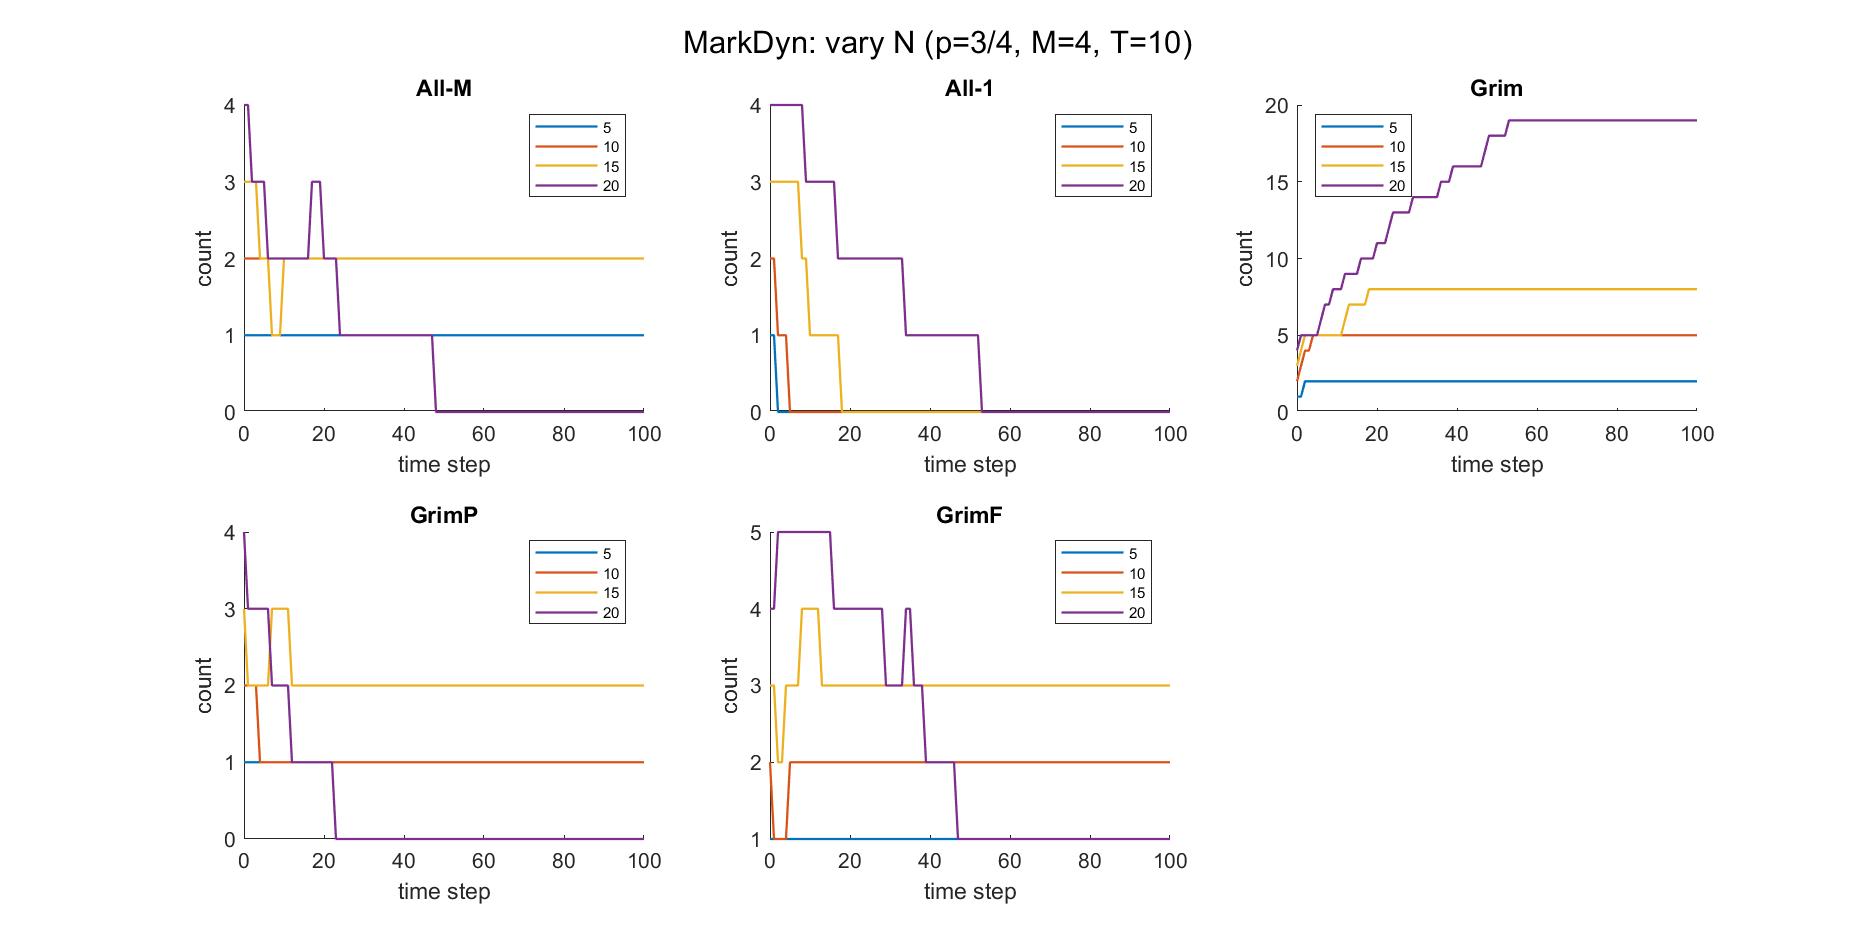
\includegraphics[width=\textwidth]{mark_overlay_vary_N}\\
      \centering\small Vary $N$: larger population slows drift but same long-run outcome.
  \end{columns}
\end{frame}

%============================================================
\section{Comparing Grim Variants}
%============================================================

\begin{frame}{Comparing the Three Grim Variants}
  All three earn $TM$ against cooperators --- they differ only in how exploitable they are by All-$1$.

  \begin{center}
  \begin{tabular}{lccc}
    \toprule
    Strategy & Trigger condition & All-$1$ earns & \\ 
    \midrule
    Grim          & 1st defection (permanent)     & $C(2,3) = 11.25$ & least exploitable \\
    Grim-Patient  & 2 consecutive (permanent)     & $C(2,4) = 12.5$  & \\
    Grim-Forgiver & 1st defection, forgive after 2 & $C(2,5) = 15.0$  & most exploitable  \\
    \bottomrule
  \end{tabular}
  \end{center}

  \vspace{6pt}
  \textbf{Why GrimF is most exploitable:}\\
  GrimF cycles $[\rho_M, \rho_1, \rho_1, \rho_M, \rho_1, \rho_1, \ldots]$ when facing All-$1$.
  It returns to full cooperation every 3 rounds, allowing All-$1$ to exploit it repeatedly.

  \vspace{6pt}
  \textbf{Trade-off:} Grim is harshest and least exploitable, but GrimF allows partial cooperation recovery after punishment --- a softer but more vulnerable approach.
\end{frame}

%============================================================
\section{Conclusions}
%============================================================

\begin{frame}{Conclusions}
  \begin{enumerate}
    \item \textbf{Payoff degeneracy.}
      All cooperating strategies earn $TM$ against each other $\Rightarrow$ continuum of Nash equilibria among cooperators.
    \item \textbf{Critical threshold $p^* = 2/3$.}
      Cooperation survives evolution if and only if $p < 2/3$.
    \item \textbf{No ESS among cooperators.}
      Neutral drift, not selection, determines the long-run mix of All-$M$ / Grim / GrimP / GrimF.
    \item \textbf{GrimF is most exploitable.}
      Its periodic forgiveness allows All-$1$ to extract full cooperation repeatedly.
      Grim is the most resistant to exploitation.
    \item \textbf{Markov dynamics.}
      The absorbing face $\mathcal{A} = \{s_2 = 0\}$ captures the long-run cooperative outcome.
      Convergence to cooperation or All-$1$ depends on $p$ and initial conditions.
    \item \textbf{Learning interpretation.}
      PPI $\equiv$ social imitation; replicator $\equiv$ reinforcement learning.
      Both frameworks converge to the same $p^*$-threshold behavior.
  \end{enumerate}
\end{frame}

\begin{frame}{Future Work}
  \begin{itemize}
    \item Add \textbf{Tit-for-Tat} and \textbf{Generous-Tit-for-Tat} to the strategy set.
    \item Study the effect of \textbf{noise/mutation} on the neutrally stable cooperative face.
    \item Analyse \textbf{asymmetric populations} via two-population replicator dynamics.
  \end{itemize}
  \vspace{20pt}
  \begin{center}
    \large Thank you --- Questions?
  \end{center}
\end{frame}

%============================================================
\end{document}
%============================================================